\documentclass{article}

\usepackage{graphicx}
\usepackage{tikz}
\usepackage{tikzsymbols}
\usetikzlibrary{calc,patterns,shapes.geometric}
\pagestyle{empty}
\usepackage[margin=0pt]{geometry}
\geometry{papersize={14in,12in}}

\def\centerarc[#1](#2)(#3:#4:#5){\draw[#1] ($(#2)+({#5*cos(#3)},{#5*sin(#3)})$) arc (#3:#4:#5);}

\begin{document}
	\begin{figure}
		\centering
		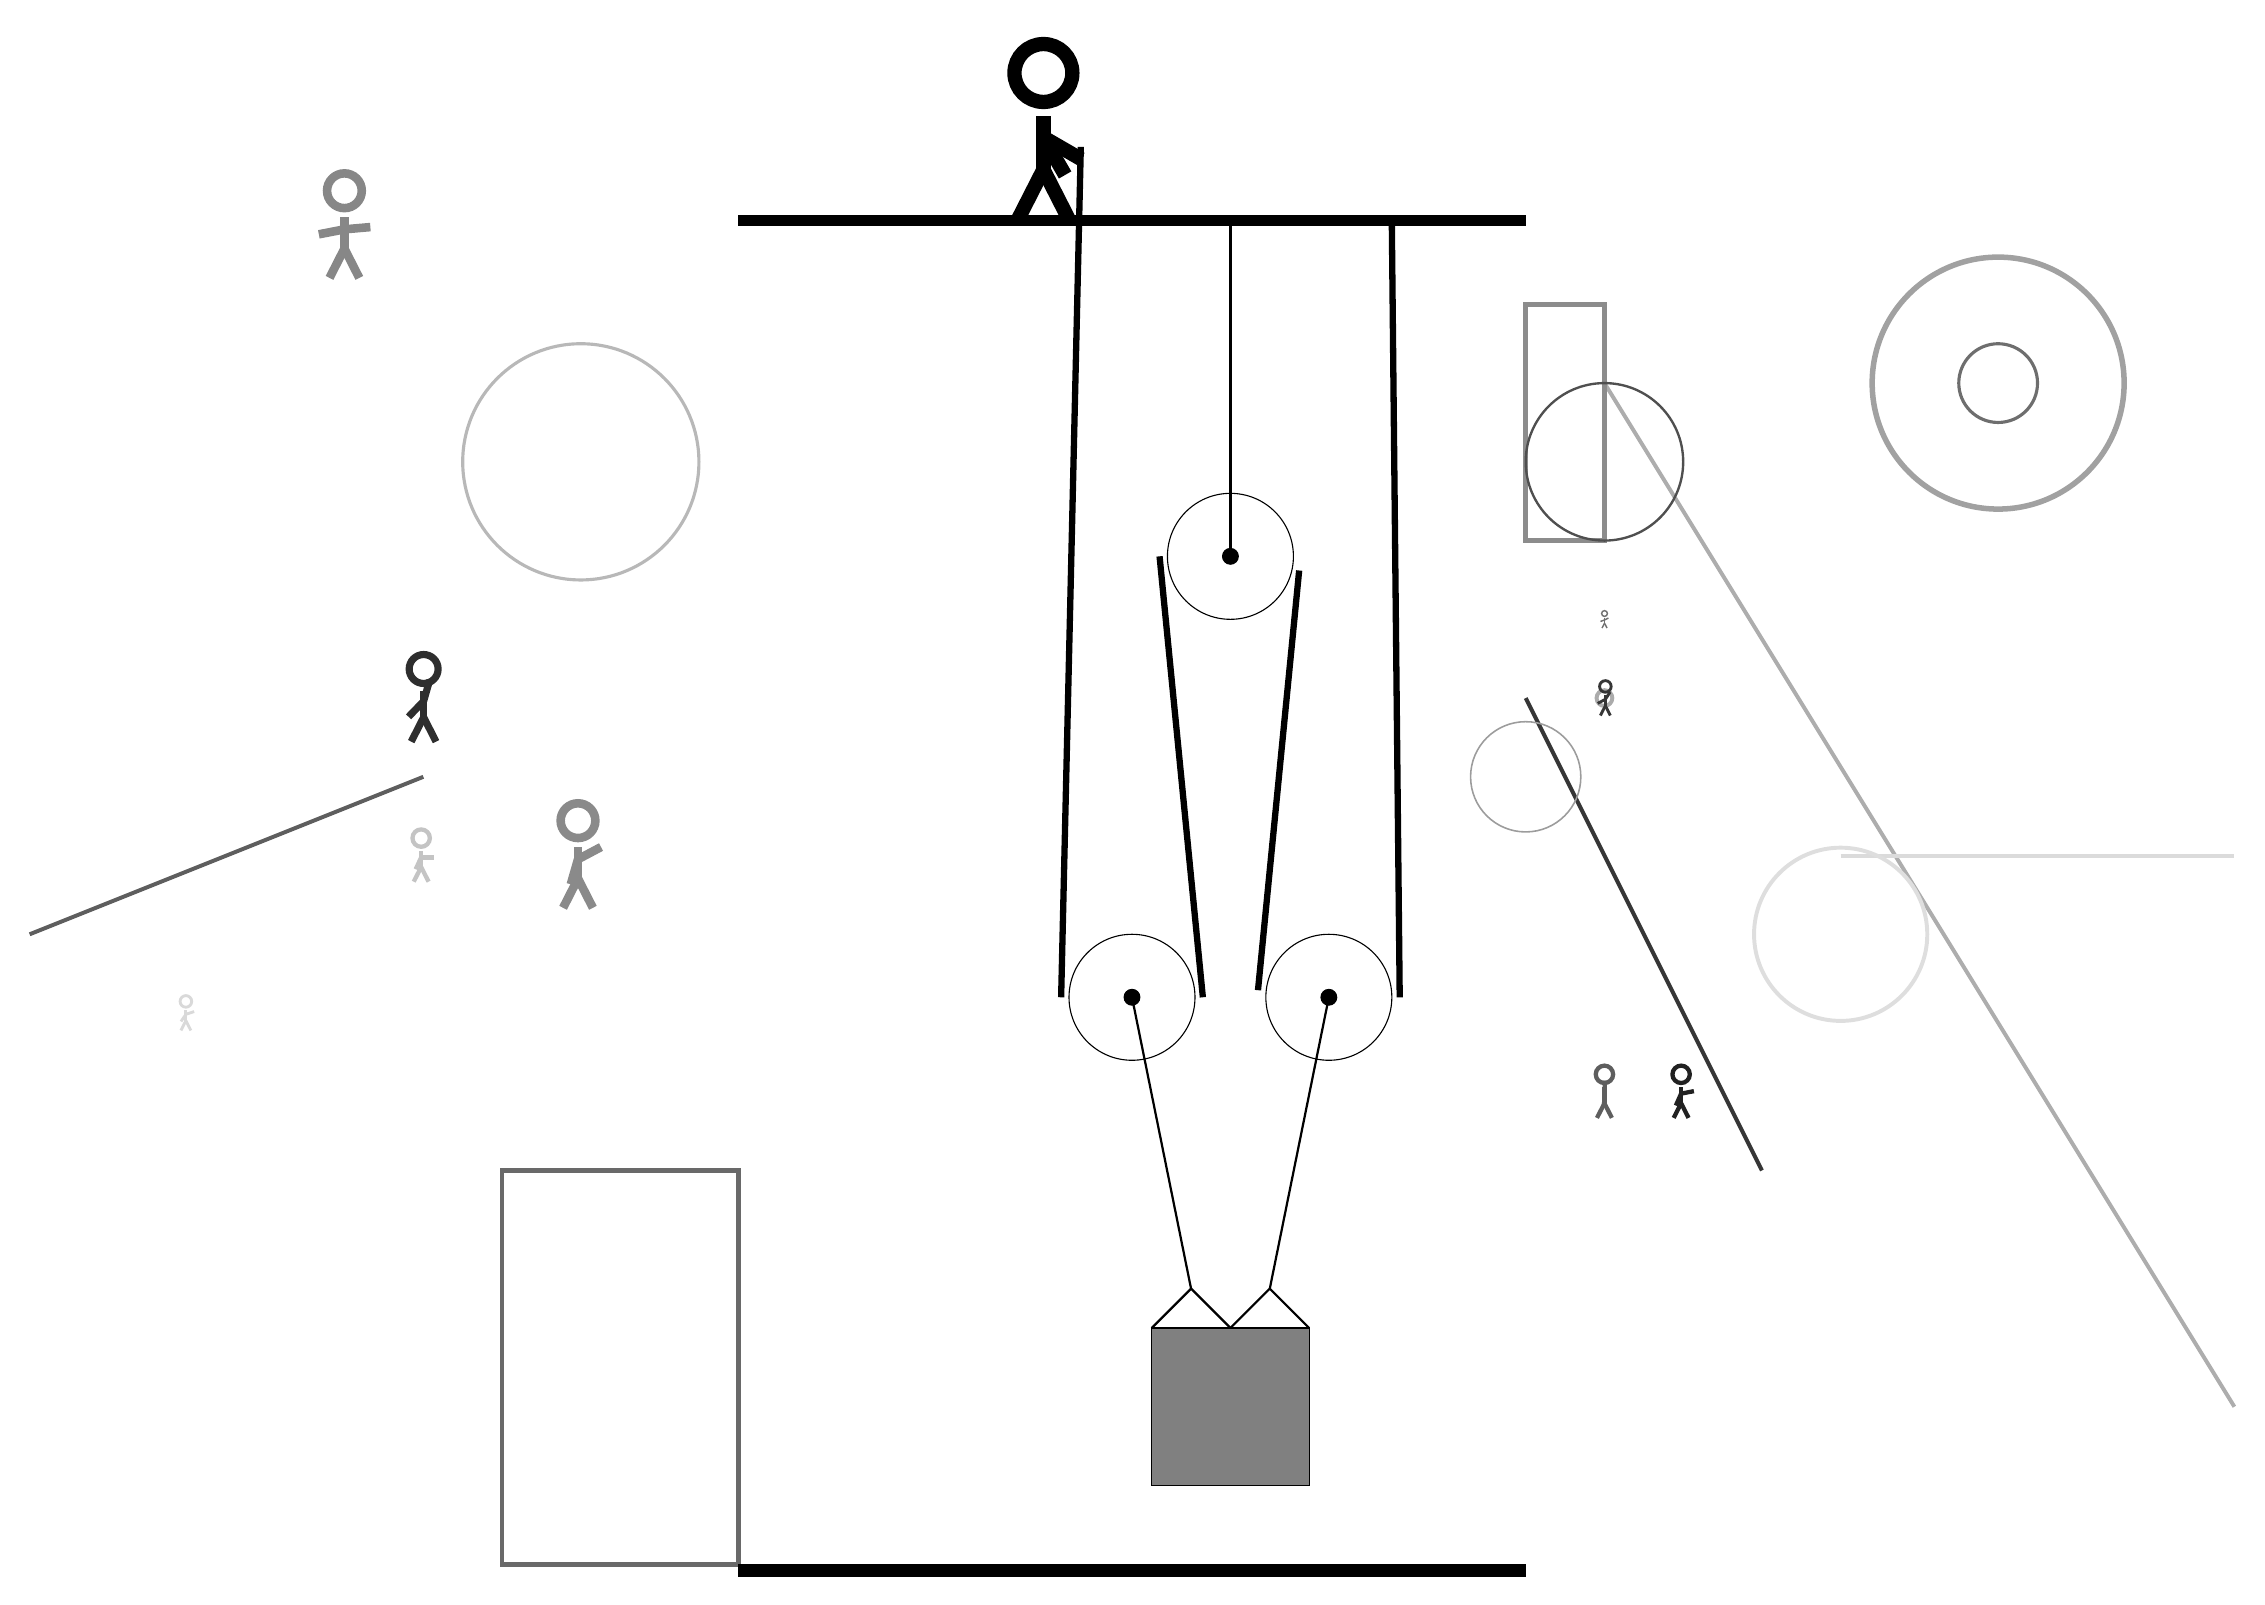
\begin{tikzpicture}
			%%%%% START %%%%%
			
			\draw[fill=black] (-4, 14) rectangle (6, 14.125);
			
			\draw (1, 4.2) circle (0.8);
			\draw[fill=black] (1, 4.2) circle (0.1);
			
			\draw[line width=0.5mm, color=black!32](7, 12) -- (15, -1);
			
			\draw [line width=0.5mm, color=black!33](7, 8) circle (0.1);
			\node[line width=0.2mm, color=black!23] at (-8, 6) {\Strichmaxerl[3][65][0]};
			\node[line width=0.6mm, color=black!15] at (-11, 4) {\Strichmaxerl[2][56][18]};
			
			\node[line width=0.3mm, color=black!79] at (7, 8) {\Strichmaxerl[2][28][57]};
			
			\node[line width=0.3mm, color=black!46] at (-6, 6) {\Strichmaxerl[6][74][28]};
			
			\draw[line width=0.7mm, color=black!45] (7, 13) rectangle (6, 10);
			
			\node[line width=0.2mm, color=black!63] at (7, 3) {\Strichmaxerl[3][88][88]};
			\draw[line width=0.5mm, color=black!14](10, 6) -- (15, 6);
			\node[line width=0.3mm, color=black!87] at (8, 3) {\Strichmaxerl[3][66][11]};
			
			\node[line width=0.2mm, color=black!47] at (-9, 14) {\Strichmaxerl[6][11][5]};
			\draw [line width=0.7mm, color=black!36](9, 12) circle (0.0);
			\draw[line width=0.5mm, color=black!79](9, 2) -- (6, 8);
			
			\draw [line width=0.4mm, color=black!28](-6, 11) circle (1.5);
			\node[line width=0.2mm, color=black!56] at (7, 9) {\Strichmaxerl[1][21][26]};
			\draw [line width=0.3mm, color=black!69](7, 11) circle (1.0);
			\draw [line width=0.4mm, color=black!57](12, 12) circle (0.5);
			
			\draw [line width=0.7mm, color=black!37](12, 12) circle (1.6);
			\draw[line width=0.6mm, color=black!59] (-4, 2) rectangle (-7, -3);
			\draw [line width=0.5mm, color=black!13](10, 5) circle (1.1);
			\draw [line width=0.2mm, color=black!39](6, 7) circle (0.7);
			\draw[line width=0.5mm, color=black!63](-8, 7) -- (-13, 5);
			\node[line width=0.3mm, color=black!82] at (-8, 8) {\Strichmaxerl[5][46][74]};
			
			\draw (2.25, 9.8) circle (0.8);
			\draw[fill=black] (2.25, 9.8) circle (0.1);
			\draw[thick] (2.25, 9.8) -- (2.25, 14);
			
			\draw (3.5, 4.2) circle (0.8);
			\draw[fill=black] (3.5, 4.2) circle (0.1);
			
			\draw[thick] (3.5, 4.2) -- (2.75, 0.5);
			\draw[thick] (1, 4.2) -- (1.75, 0.5);
			\draw[thick]  (1.25, 0) -- (1.75, 0.5) -- (2.25, 0);
			\draw[thick]  (2.25, 0) -- (2.75, 0.5) -- (3.25, 0);
			\draw[fill=black!50] (1.25, 0) rectangle (3.25, -2);
			
			\draw[line width=0.8mm] (0.35, 15) --  (0.1, 4.2);
			\centerarc[line width=0.8mm](1, 4.2)(180:360:0.9);
			\draw[line width=0.8mm] (1.9, 4.2) -- (1.35, 9.8);
			\centerarc[line width=0.8mm](2.25, 9.8)(-20:180:0.9);
			\draw[line width=0.8mm](3.123, 9.62) -- (2.6, 4.29);
			\centerarc[line width=0.8mm](3.5, 4.2)(160:360:0.9);
			\draw[line width=0.8mm](4.4, 4.2) -- (4.3, 14);
			
			\node at (-0.07, 15.2) {\Strichmaxerl[10][120][-30]};
			
			\draw[fill=black] (-4, -3) rectangle (6, -3.15);
			
			%%%%% END %%%%%
		\end{tikzpicture}
	\end{figure}	
\end{document}